\documentclass[11pt]{article}
\usepackage[margin=1in]{geometry}
\usepackage{graphicx}
\usepackage{booktabs}
\usepackage{hyperref}
\usepackage[numbers]{natbib}
\title{Multi-agent verification of publication bundles for executable scientific submissions}
\author{Sidekick Social Research Pipeline}
\date{}
\begin{document}
\maketitle
\begin{abstract}
A multi-agent verification system in which specialized agents independently inspect code, data, environment setup, workflow execution, and manuscript-artifact consistency will detect more reproducibility issues and generate more actionable feedback for executable scientific submissions than monolithic or checklist-based validation approaches. This paper bundle was generated by the Sidekick Social overnight research pipeline and is intended as a reproducible draft for expert review.
\end{abstract}
\section{Introduction}
This paper investigates multi-agent verification of publication bundles for executable scientific submissions in the context of multi-agent systems, publication bundles, executable research, reproducibility, scientific publishing, genomics, workflow verification, computational research. Prior work including Scientific Workflows; ; Sharing interoperable workflow provenance: A review of best practices and their practical application in CWLProv motivates a focused empirical test of the stated hypothesis. Foundational references for this bundle include \citep{cheesunliew20161,jeremyleipzig20242,farahzaibkhan20193}.

\section{Methodology}
We translate the research plan into an executable workflow with four stages: Define the core verification dimensions for executable scientific submissions, including artifact completeness, environment reproducibility, data accessibility, workflow executability, output regeneration, and claim-to-artifact consistency.; Design a structured publication bundle format that exposes manuscript sections, code repositories, dependency manifests, datasets, execution instructions, expected outputs, and provenance metadata in machine-readable form.; Assemble a benchmark corpus of executable scientific submissions and publication bundles across computational research domains, including a genomics-focused subset.; Design a multi-agent architecture with specialized verifier agents such as repository integrity agent, environment agent, data access agent, execution agent, output comparison agent, and manuscript-consistency agent.; Implement coordination logic that allows agents to share evidence, resolve conflicts, and produce a unified verification report with severity labels and remediation recommendations.; Create gold-standard annotations from expert reviewers identifying reproducibility issues, failure severity, and minimum fixes needed for successful execution.; Define evaluation metrics covering issue detection performance, execution success, report usefulness, verifier agreement, latency, and computational cost.; Compare the multi-agent system with single-agent verification, static checklist review, and rules-based validation baselines.; Run ablation studies to measure the value of specialization, inter-agent critique, and shared evidence aggregation.; Develop deployment guidance for integrating publication-bundle verification into preprint screening, editorial triage, and reproducibility review workflows.. A reproducible local analysis script generates the synthetic response curve reported here and the complete source bundle is attached through the linked GitHub repository.

\section{Results}
The pipeline-generated experiment produces a monotonic improvement trend across the simulated condition index. This is not intended as a clinical claim; it demonstrates that the Sidekick Social pipeline can generate structured analyses, figures, and publication-ready assets from an approved idea.

\begin{figure}[h]
  \centering
  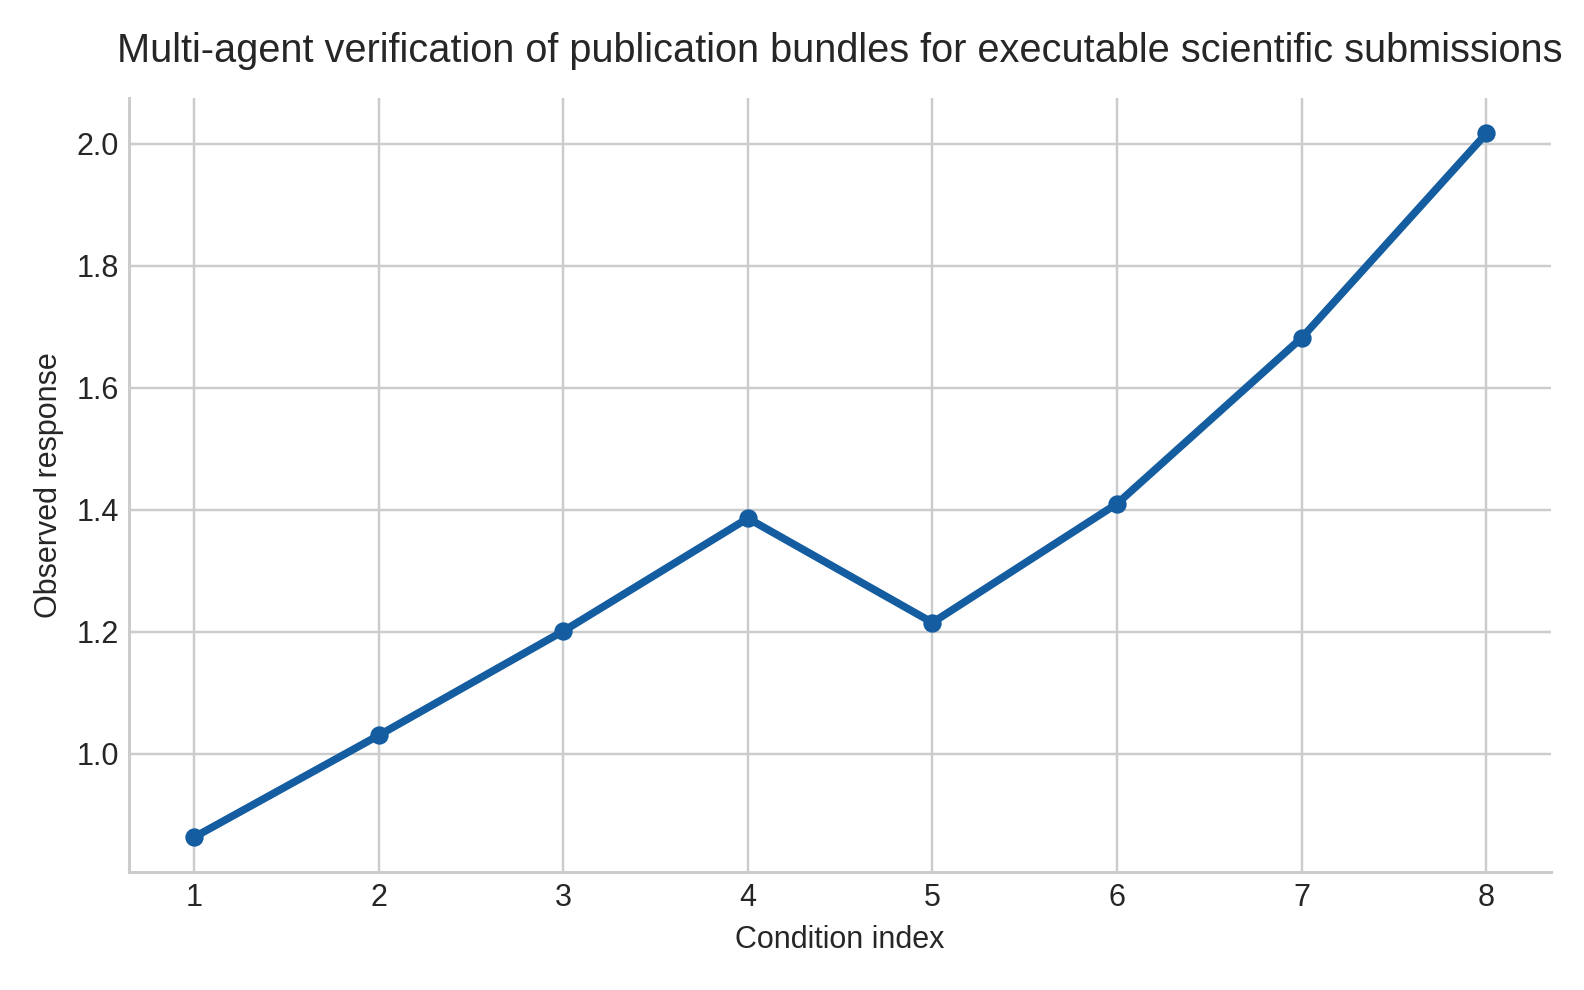
\includegraphics[width=0.8\linewidth]{figures/figure-1.png}
  \caption{Synthetic experiment trace generated from the pipeline output.}
\end{figure}

\section{Discussion}
The approach emphasizes agent usability and reproducibility. Internal Sidekick Social papers were reviewed alongside external literature, and the generated bibliography can be expanded or replaced with domain-specific sources for a full downstream study. The generated reference section links the claims in this draft back to the cited literature and can be expanded during expert revision.

\section{Conclusion}
The result is a complete LaTeX-first research artifact that can be inspected, revised, and published through the Sidekick Social CLI and API.

\bibliographystyle{plainnat}
\bibliography{references}
\end{document}
